\documentclass[12pt]{article}
\usepackage[table]{xcolor}
\usepackage[shortlabels]{enumitem}
\usepackage{tabularx,xltabular}
\usepackage{graphicx}
\usepackage{hyperref}
\usepackage{verbatim}
\usepackage{geometry}
\usepackage{ulem}
\usepackage[official]{eurosym}
\usepackage{tikz}
\usetikzlibrary{arrows,backgrounds,calc,decorations.markings,patterns,3d}
\usepackage{pgfplots}
\pgfplotsset{compat = newest}
\usetikzlibrary{fit}
\newcommand\addvmargin[1]{
\usetikzlibrary{arrows}
\node[fit=(current bounding box),inner ysep=#1,inner xsep=0]{};}
\usepackage{cancel}
\usepackage{fontspec}
\usepackage{array}  
\geometry{a4paper, top=2cm, left=2cm, right=2cm, bottom=2cm, headsep=1cm}
\usepackage{tabu}
\usepackage{pst-node}
\usepackage{colortbl}
\usepackage{array}
\usepackage{german}
\setlength\parindent{0pt}
\newcolumntype{?}{!{\vrule width 1pt}}
\usepackage{makecell}
\renewcommand{\arraystretch}{2.5}
\usepackage{pbox}
\usepackage{amssymb}
\usepackage{amsmath}
\usepackage{booktabs}
\newcolumntype{L}[1]{>{\raggedright\let\newline\\\arraybackslash\hspace{0pt}}m{#1}}
\newcolumntype{C}[1]{>{\centering\let\newline\\\arraybackslash\hspace{0pt}}m{#1}}
\newcolumntype{R}[1]{>{\raggedleft\let\newline\\\arraybackslash\hspace{0pt}}m{#1}}
\begin{document}
\rightline{Datum: 08.06.2023}
\centerline{{\Large Tägliche Übungen}} 
\vspace{1cm}
\noindent \\


\begin{xltabular}{\textwidth}{|C{0.75cm}|X|C{0.75cm}|X|}
\arrayrulecolor{black}\hline
a)&$\begin{aligned}
 a=&5~ \rightarrow ~ 5 \cdot a - 3=?
\end{aligned}$
&
b)&$\begin{aligned}
 x=&4~ \rightarrow ~ 4 - 4 \cdot x=?
\end{aligned}$
\\\hline
c)&$\begin{aligned}
 a=&-10~ \rightarrow ~ 3 \cdot a + 5 \cdot a=?
\end{aligned}$
&
d)&$\begin{aligned}
 a=&-1~ \rightarrow ~ 5 \cdot a - 3 \cdot a=?
\end{aligned}$
\\\hline
e)&$a-40 = 25$
&
f)&$a-47 = 24$
\\\hline
g)&$b+19 = 42$
&
h)&$a+1 = 26$
\\\hline
i)&$a+7 = 9$
&
j)&$b-49 = 33$
\\\hline
k)&$b-1 = 45$
&
l)&$y+7 = 40$
\\\hline
m)&$a-15 = 38$
&
n)&$b+36 = 42$
\\\hline
o)&$y-11 = 6$
&
p)&$a-17 = 17$
\\\hline
q)&$a-17 = 43$
&
r)&$b+9 = 10$
\\\hline
s)&$y-36 = 4$
&
t)&$b+50 = 16$
\\\hline
u)&$y-6 = 3$
&
v)&$y+24 = 42$
\\\hline
w)&$b+26 = 16$
&
x)&$y+29 = 46$
\\\hline
y)&$x-3 = 9$
&
z)&$x+24 = 19$
\\\hline
\end{xltabular}
\vspace{0.5cm}
\newpage
\rightline{Datum: 08.06.2023}
\centerline{{\large Lösungen Tägliche Übungen}} 
\vspace{0.5cm}

\begin{xltabular}{\textwidth}{|C{0.75cm}|X|C{0.75cm}|X|}
\arrayrulecolor{black}\hline
a)&$\begin{aligned}
\textcolor{red}{a=5} & \rightarrow\\
5 \cdot a - 3=&5 \cdot \textcolor{red}{5} - 3=22\\
\end{aligned}$
&
b)&$\begin{aligned}
\textcolor{red}{x=4} & \rightarrow\\
4 - 4 \cdot x=&4 - 4 \cdot \textcolor{red}{4}=-12\\
\end{aligned}$
\\\hline
c)&$\begin{aligned}
\textcolor{red}{a=-10} & \rightarrow\\
3 \cdot a + 5 \cdot a=&3 \cdot \textcolor{red}{(-10)} + 5 \cdot \textcolor{red}{(-10)}=-80\\
\end{aligned}$
&
d)&$\begin{aligned}
\textcolor{red}{a=-1} & \rightarrow\\
5 \cdot a - 3 \cdot a=&5 \cdot \textcolor{red}{(-1)} - 3 \cdot \textcolor{red}{(-1)}=-2\\
\end{aligned}$
\\\hline
e)&\begingroup\setlength{\jot}{-0.03cm}
\tikzstyle{background grid}=[draw, black!15,step=.5cm]
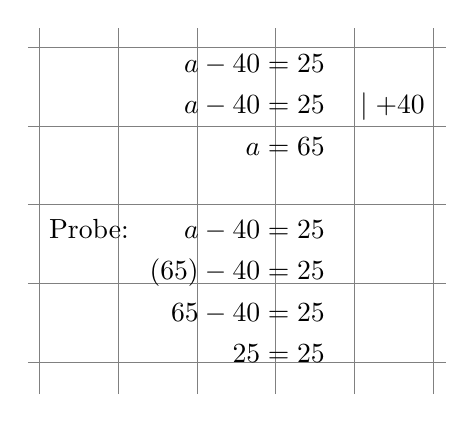
\begin{tikzpicture}[show background grid]
\node[below right] at (0,0.1) {
$\begin{aligned}
a-40  &= 25& &  \\
a - 40 &=25& & \mid + 40\\
a &=65& & 
\\
\\
\mbox{Probe:}\qquad a-40  &= 25& &  \\
\left(65\right)-40  &= 25& &  \\
65-40 &=25& &  \\
25 &=25& &  \\
\end{aligned}$};
\end{tikzpicture}
\endgroup
&
f)&\begingroup\setlength{\jot}{-0.03cm}
\tikzstyle{background grid}=[draw, black!15,step=.5cm]
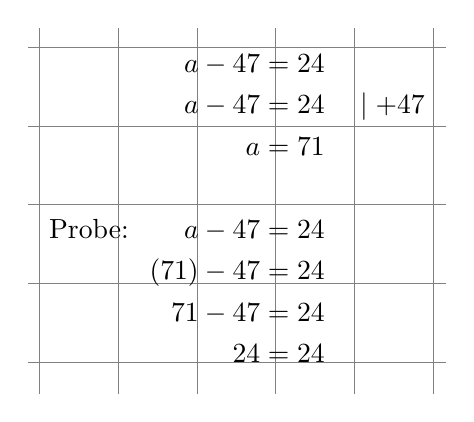
\begin{tikzpicture}[show background grid]
\node[below right] at (0,0.1) {
$\begin{aligned}
a-47  &= 24& &  \\
a - 47 &=24& & \mid + 47\\
a &=71& & 
\\
\\
\mbox{Probe:}\qquad a-47  &= 24& &  \\
\left(71\right)-47  &= 24& &  \\
71-47 &=24& &  \\
24 &=24& &  \\
\end{aligned}$};
\end{tikzpicture}
\endgroup
\\\hline
g)&\begingroup\setlength{\jot}{-0.03cm}
\tikzstyle{background grid}=[draw, black!15,step=.5cm]
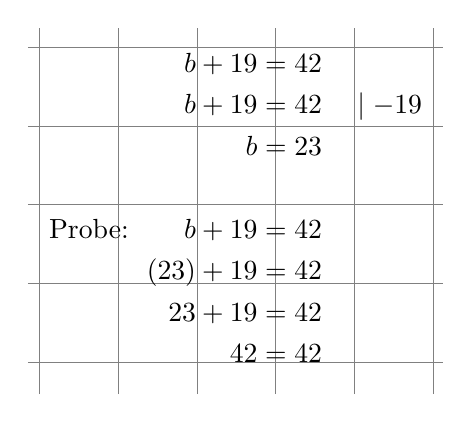
\begin{tikzpicture}[show background grid]
\node[below right] at (0,0.1) {
$\begin{aligned}
b+19  &= 42& &  \\
b + 19 &=42& & \mid - 19\\
b &=23& & 
\\
\\
\mbox{Probe:}\qquad b+19  &= 42& &  \\
\left(23\right)+19  &= 42& &  \\
23+19 &=42& &  \\
42 &=42& &  \\
\end{aligned}$};
\end{tikzpicture}
\endgroup
&
h)&\begingroup\setlength{\jot}{-0.03cm}
\tikzstyle{background grid}=[draw, black!15,step=.5cm]
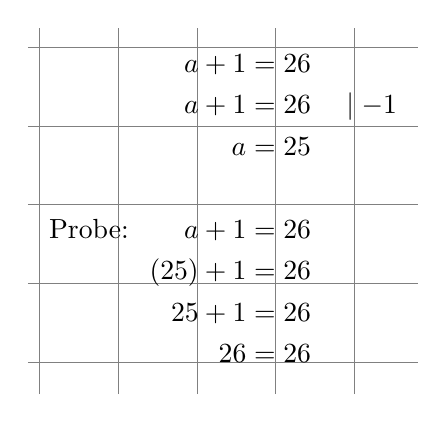
\begin{tikzpicture}[show background grid]
\node[below right] at (0,0.1) {
$\begin{aligned}
a+1  &= 26& &  \\
a + 1 &=26& & \mid - 1\\
a &=25& & 
\\
\\
\mbox{Probe:}\qquad a+1  &= 26& &  \\
\left(25\right)+1  &= 26& &  \\
25+1 &=26& &  \\
26 &=26& &  \\
\end{aligned}$};
\end{tikzpicture}
\endgroup
\\\hline
i)&\begingroup\setlength{\jot}{-0.03cm}
\tikzstyle{background grid}=[draw, black!15,step=.5cm]
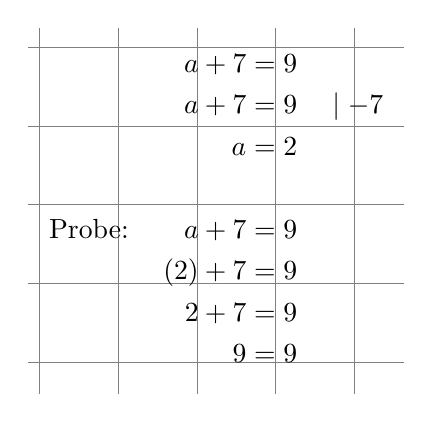
\begin{tikzpicture}[show background grid]
\node[below right] at (0,0.1) {
$\begin{aligned}
a+7  &= 9& &  \\
a + 7 &=9& & \mid - 7\\
a &=2& & 
\\
\\
\mbox{Probe:}\qquad a+7  &= 9& &  \\
\left(2\right)+7  &= 9& &  \\
2+7 &=9& &  \\
9 &=9& &  \\
\end{aligned}$};
\end{tikzpicture}
\endgroup
&
j)&\begingroup\setlength{\jot}{-0.03cm}
\tikzstyle{background grid}=[draw, black!15,step=.5cm]
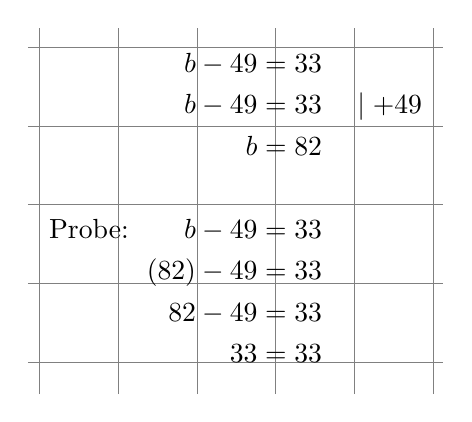
\begin{tikzpicture}[show background grid]
\node[below right] at (0,0.1) {
$\begin{aligned}
b-49  &= 33& &  \\
b - 49 &=33& & \mid + 49\\
b &=82& & 
\\
\\
\mbox{Probe:}\qquad b-49  &= 33& &  \\
\left(82\right)-49  &= 33& &  \\
82-49 &=33& &  \\
33 &=33& &  \\
\end{aligned}$};
\end{tikzpicture}
\endgroup
\\\hline
k)&\begingroup\setlength{\jot}{-0.03cm}
\tikzstyle{background grid}=[draw, black!15,step=.5cm]
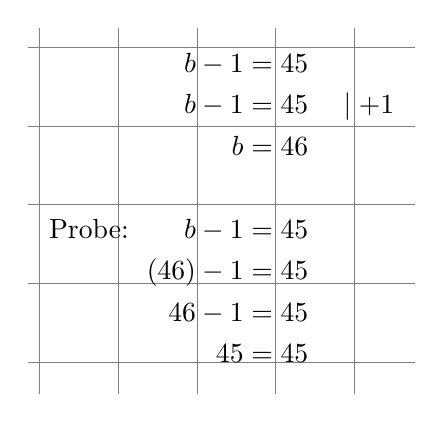
\begin{tikzpicture}[show background grid]
\node[below right] at (0,0.1) {
$\begin{aligned}
b-1  &= 45& &  \\
b - 1 &=45& & \mid + 1\\
b &=46& & 
\\
\\
\mbox{Probe:}\qquad b-1  &= 45& &  \\
\left(46\right)-1  &= 45& &  \\
46-1 &=45& &  \\
45 &=45& &  \\
\end{aligned}$};
\end{tikzpicture}
\endgroup
&
l)&\begingroup\setlength{\jot}{-0.03cm}
\tikzstyle{background grid}=[draw, black!15,step=.5cm]
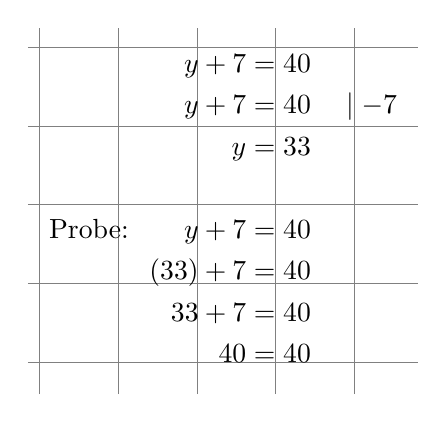
\begin{tikzpicture}[show background grid]
\node[below right] at (0,0.1) {
$\begin{aligned}
y+7  &= 40& &  \\
y + 7 &=40& & \mid - 7\\
y &=33& & 
\\
\\
\mbox{Probe:}\qquad y+7  &= 40& &  \\
\left(33\right)+7  &= 40& &  \\
33+7 &=40& &  \\
40 &=40& &  \\
\end{aligned}$};
\end{tikzpicture}
\endgroup
\\\hline
m)&\begingroup\setlength{\jot}{-0.03cm}
\tikzstyle{background grid}=[draw, black!15,step=.5cm]
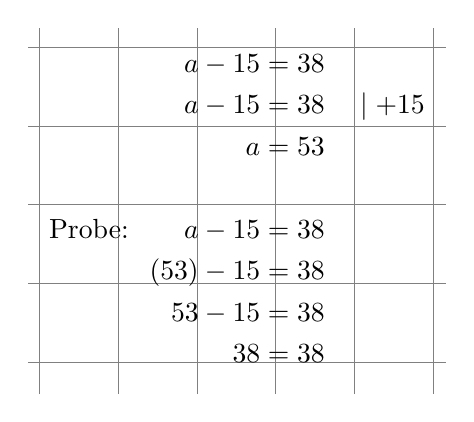
\begin{tikzpicture}[show background grid]
\node[below right] at (0,0.1) {
$\begin{aligned}
a-15  &= 38& &  \\
a - 15 &=38& & \mid + 15\\
a &=53& & 
\\
\\
\mbox{Probe:}\qquad a-15  &= 38& &  \\
\left(53\right)-15  &= 38& &  \\
53-15 &=38& &  \\
38 &=38& &  \\
\end{aligned}$};
\end{tikzpicture}
\endgroup
&
n)&\begingroup\setlength{\jot}{-0.03cm}
\tikzstyle{background grid}=[draw, black!15,step=.5cm]
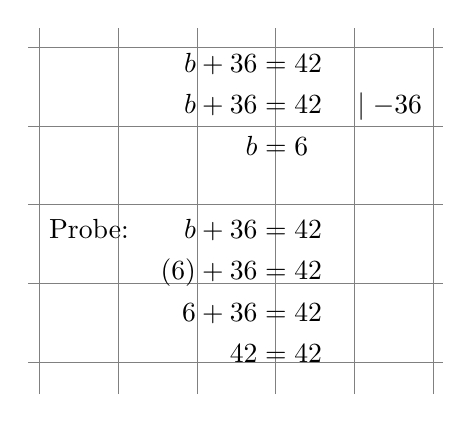
\begin{tikzpicture}[show background grid]
\node[below right] at (0,0.1) {
$\begin{aligned}
b+36  &= 42& &  \\
b + 36 &=42& & \mid - 36\\
b &=6& & 
\\
\\
\mbox{Probe:}\qquad b+36  &= 42& &  \\
\left(6\right)+36  &= 42& &  \\
6+36 &=42& &  \\
42 &=42& &  \\
\end{aligned}$};
\end{tikzpicture}
\endgroup
\\\hline
o)&\begingroup\setlength{\jot}{-0.03cm}
\tikzstyle{background grid}=[draw, black!15,step=.5cm]
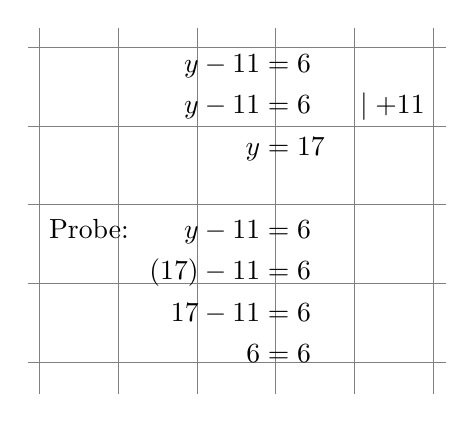
\begin{tikzpicture}[show background grid]
\node[below right] at (0,0.1) {
$\begin{aligned}
y-11  &= 6& &  \\
y - 11 &=6& & \mid + 11\\
y &=17& & 
\\
\\
\mbox{Probe:}\qquad y-11  &= 6& &  \\
\left(17\right)-11  &= 6& &  \\
17-11 &=6& &  \\
6 &=6& &  \\
\end{aligned}$};
\end{tikzpicture}
\endgroup
&
p)&\begingroup\setlength{\jot}{-0.03cm}
\tikzstyle{background grid}=[draw, black!15,step=.5cm]
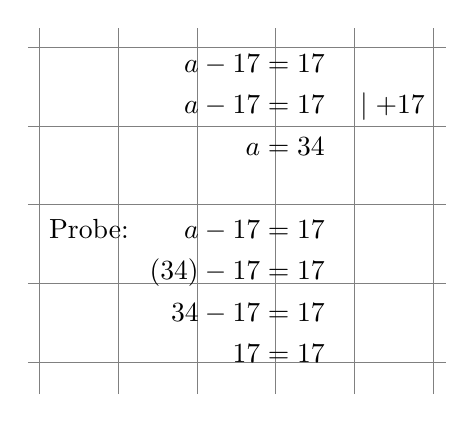
\begin{tikzpicture}[show background grid]
\node[below right] at (0,0.1) {
$\begin{aligned}
a-17  &= 17& &  \\
a - 17 &=17& & \mid + 17\\
a &=34& & 
\\
\\
\mbox{Probe:}\qquad a-17  &= 17& &  \\
\left(34\right)-17  &= 17& &  \\
34-17 &=17& &  \\
17 &=17& &  \\
\end{aligned}$};
\end{tikzpicture}
\endgroup
\\\hline
q)&\begingroup\setlength{\jot}{-0.03cm}
\tikzstyle{background grid}=[draw, black!15,step=.5cm]
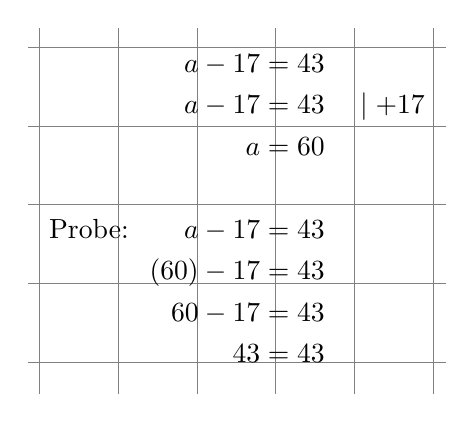
\begin{tikzpicture}[show background grid]
\node[below right] at (0,0.1) {
$\begin{aligned}
a-17  &= 43& &  \\
a - 17 &=43& & \mid + 17\\
a &=60& & 
\\
\\
\mbox{Probe:}\qquad a-17  &= 43& &  \\
\left(60\right)-17  &= 43& &  \\
60-17 &=43& &  \\
43 &=43& &  \\
\end{aligned}$};
\end{tikzpicture}
\endgroup
&
r)&\begingroup\setlength{\jot}{-0.03cm}
\tikzstyle{background grid}=[draw, black!15,step=.5cm]
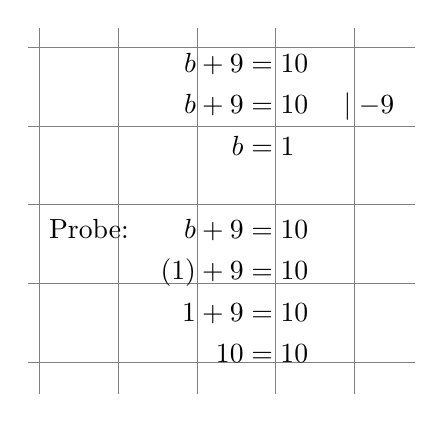
\begin{tikzpicture}[show background grid]
\node[below right] at (0,0.1) {
$\begin{aligned}
b+9  &= 10& &  \\
b + 9 &=10& & \mid - 9\\
b &=1& & 
\\
\\
\mbox{Probe:}\qquad b+9  &= 10& &  \\
\left(1\right)+9  &= 10& &  \\
1+9 &=10& &  \\
10 &=10& &  \\
\end{aligned}$};
\end{tikzpicture}
\endgroup
\\\hline
s)&\begingroup\setlength{\jot}{-0.03cm}
\tikzstyle{background grid}=[draw, black!15,step=.5cm]
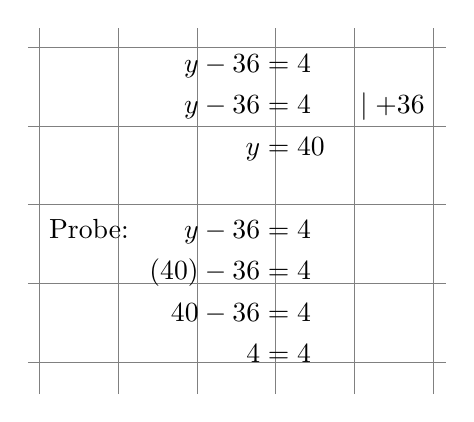
\begin{tikzpicture}[show background grid]
\node[below right] at (0,0.1) {
$\begin{aligned}
y-36  &= 4& &  \\
y - 36 &=4& & \mid + 36\\
y &=40& & 
\\
\\
\mbox{Probe:}\qquad y-36  &= 4& &  \\
\left(40\right)-36  &= 4& &  \\
40-36 &=4& &  \\
4 &=4& &  \\
\end{aligned}$};
\end{tikzpicture}
\endgroup
&
t)&\begingroup\setlength{\jot}{-0.03cm}
\tikzstyle{background grid}=[draw, black!15,step=.5cm]
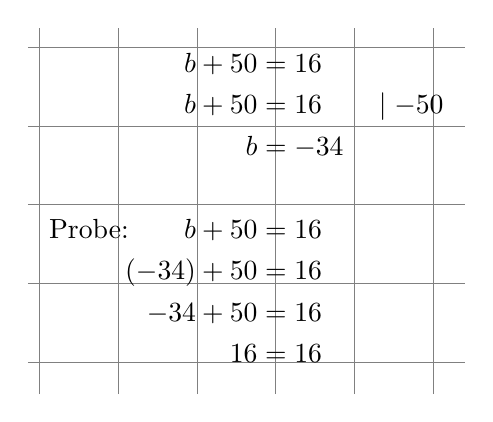
\begin{tikzpicture}[show background grid]
\node[below right] at (0,0.1) {
$\begin{aligned}
b+50  &= 16& &  \\
b + 50 &=16& & \mid - 50\\
b &=-34& & 
\\
\\
\mbox{Probe:}\qquad b+50  &= 16& &  \\
\left(-34\right)+50  &= 16& &  \\
-34+50 &=16& &  \\
16 &=16& &  \\
\end{aligned}$};
\end{tikzpicture}
\endgroup
\\\hline
u)&\begingroup\setlength{\jot}{-0.03cm}
\tikzstyle{background grid}=[draw, black!15,step=.5cm]
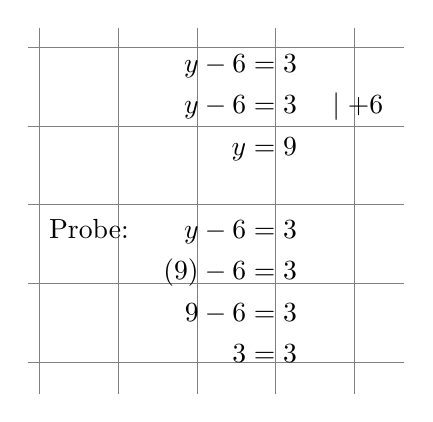
\begin{tikzpicture}[show background grid]
\node[below right] at (0,0.1) {
$\begin{aligned}
y-6  &= 3& &  \\
y - 6 &=3& & \mid + 6\\
y &=9& & 
\\
\\
\mbox{Probe:}\qquad y-6  &= 3& &  \\
\left(9\right)-6  &= 3& &  \\
9-6 &=3& &  \\
3 &=3& &  \\
\end{aligned}$};
\end{tikzpicture}
\endgroup
&
v)&\begingroup\setlength{\jot}{-0.03cm}
\tikzstyle{background grid}=[draw, black!15,step=.5cm]
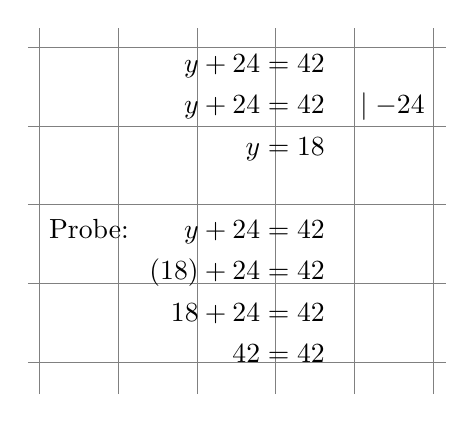
\begin{tikzpicture}[show background grid]
\node[below right] at (0,0.1) {
$\begin{aligned}
y+24  &= 42& &  \\
y + 24 &=42& & \mid - 24\\
y &=18& & 
\\
\\
\mbox{Probe:}\qquad y+24  &= 42& &  \\
\left(18\right)+24  &= 42& &  \\
18+24 &=42& &  \\
42 &=42& &  \\
\end{aligned}$};
\end{tikzpicture}
\endgroup
\\\hline
w)&\begingroup\setlength{\jot}{-0.03cm}
\tikzstyle{background grid}=[draw, black!15,step=.5cm]
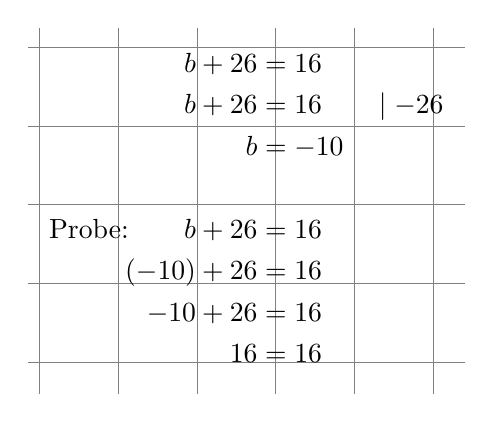
\begin{tikzpicture}[show background grid]
\node[below right] at (0,0.1) {
$\begin{aligned}
b+26  &= 16& &  \\
b + 26 &=16& & \mid - 26\\
b &=-10& & 
\\
\\
\mbox{Probe:}\qquad b+26  &= 16& &  \\
\left(-10\right)+26  &= 16& &  \\
-10+26 &=16& &  \\
16 &=16& &  \\
\end{aligned}$};
\end{tikzpicture}
\endgroup
&
x)&\begingroup\setlength{\jot}{-0.03cm}
\tikzstyle{background grid}=[draw, black!15,step=.5cm]
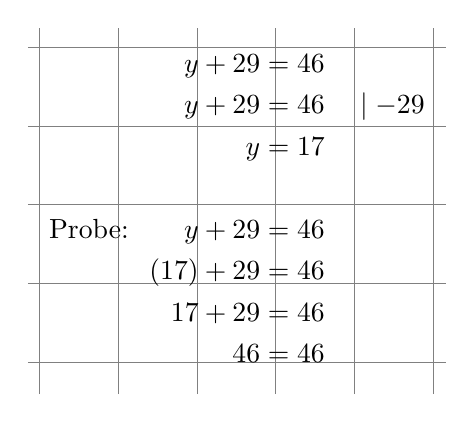
\begin{tikzpicture}[show background grid]
\node[below right] at (0,0.1) {
$\begin{aligned}
y+29  &= 46& &  \\
y + 29 &=46& & \mid - 29\\
y &=17& & 
\\
\\
\mbox{Probe:}\qquad y+29  &= 46& &  \\
\left(17\right)+29  &= 46& &  \\
17+29 &=46& &  \\
46 &=46& &  \\
\end{aligned}$};
\end{tikzpicture}
\endgroup
\\\hline
y)&\begingroup\setlength{\jot}{-0.03cm}
\tikzstyle{background grid}=[draw, black!15,step=.5cm]
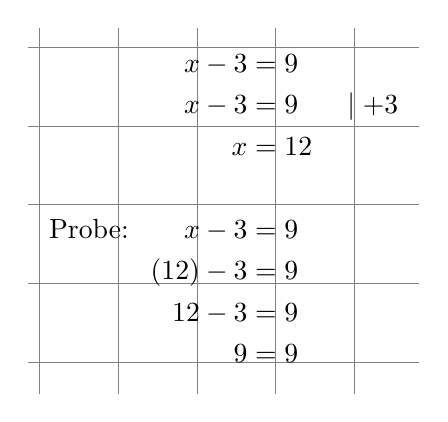
\begin{tikzpicture}[show background grid]
\node[below right] at (0,0.1) {
$\begin{aligned}
x-3  &= 9& &  \\
x - 3 &=9& & \mid + 3\\
x &=12& & 
\\
\\
\mbox{Probe:}\qquad x-3  &= 9& &  \\
\left(12\right)-3  &= 9& &  \\
12-3 &=9& &  \\
9 &=9& &  \\
\end{aligned}$};
\end{tikzpicture}
\endgroup
&
z)&\begingroup\setlength{\jot}{-0.03cm}
\tikzstyle{background grid}=[draw, black!15,step=.5cm]
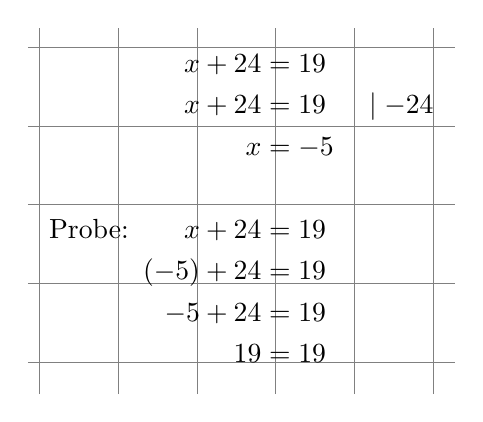
\begin{tikzpicture}[show background grid]
\node[below right] at (0,0.1) {
$\begin{aligned}
x+24  &= 19& &  \\
x + 24 &=19& & \mid - 24\\
x &=-5& & 
\\
\\
\mbox{Probe:}\qquad x+24  &= 19& &  \\
\left(-5\right)+24  &= 19& &  \\
-5+24 &=19& &  \\
19 &=19& &  \\
\end{aligned}$};
\end{tikzpicture}
\endgroup
\\\hline
\end{xltabular}
\vspace{0.5cm}
\end{document}